\chapter{Konzept}
\label{Konzept}
Im folgenden Kapitel wird das entwickelte Konzept zur Erweiterung des Testsystems (\cite{Weber2018}) beschrieben. Das Konzept wurde entwickelt, um anhand der in \autoref{Analyse} gewonnenen Erkenntnisse, verschiedene Angriffsformen in einer Industrie 4.0 Netzwerkumgebungen und deren Einfluss auf das System und die Netzwerkkommunikation demonstrieren zu können. Da die entstehende Integration und Implementierung des Konzepts für Test- und Lehrzwecke genutzt werden soll, in Zukunft um weitere Funktionalitäten erweitert werden soll und flexibel Einsetzbar sein soll, stehen die Aspekte Portabilität, Skalierbarkeit und Erweiterbarkeit bei der Entwicklung des Konzepts im Vordergrund.

Das Konzept beinhaltet die Darstellung der Verteilungs-, Baustein- und Laufzeitsicht. Dabei wird die entwickelte Netzwerkinfrastruktur, die einzelnen Komponenten sowie die Gesamtfunktionalität des Systems beschrieben.

Um eine ganzheitliche Infrastruktur mit den grundlegenden Netzwerkdiensten bereitstellen zu können, kann die Kommunikation der Systeme nicht auf der Abstraktionsebene des Docker Containernetzwerks stattfinden. Das \ac{IPAM} im Netzwerk sowie die gewünschten Dienste \ac{DHCP} und \ac{DNS} können dort nicht ausreichend konfiguriert werden. Es mussten im Laufe der Entwicklung, aufgrund des gegebenen Systems und der genutzten Software, mehrere Konzepte zur Umsetzung verschiedener Anwendungsszenarien verworfen werden. Diese werden in \autoref{Konzept:verworfene Konzepte} kurz beschrieben. Die Softwarebeschränkungen und deren Auswirkungen auf die Umsetzung des Konzepts sowie der Integration werden in \autoref{Konzept:Anpassungen} erläutert.

\section{Verteilungssicht}
Die Skalierbarkeit und Erweiterbarkeit des Testsystems wird auf der Verteilungssicht durch die Nutzung einer \ac{VM} und deren Docker Container realisiert. Um die Heterogenität des Systems gering zu halten, jedoch ein vollwertiges Netzwerk abbilden zu können, werden der vorhandenen Grundstruktur des Testsystems (\cite{Weber2018}) \ac{VM} zwei weitere Maschinen hinzugefügt.

Die \ac{VM}s simulieren, im Gegensatz zur Containervirtualisierung ein vollständiges System sowie dessen Hardware. Dies ermöglicht eine weitgehende Kontrolle über die Netzwerkschnittstellen und die Konfiguration gekapselter Netzwerkinfrastrukturen. Diese Vorteile werden genutzt, um die Netzwerkkommunikation mit Hilfe von virtuellen, internen Netzwerken auf der Abstraktionsebene der \ac{VM}s durchzuführen.

Das Konzept der Netzwerkinfrastruktur ist in \autoref{Konzept:Netzwerkkonzept} in Anlehnung an ein \ac{UML}-Verteilungsdiagramm dargestellt. Zur Umsetzung der in \autoref{Anwendungsszenarien} beschrieben Szenarien, ist es notwendig den Netzwerkdienst \ac{DHCP} bereitzustellen. Dieser wird, zusammen mit dem Dienst \ac{DNS} im Netzwerk "`i40-network"' bereitgestellt. Das zusätzliche Netzwerk "`i40-monitoring"' wird genutzt, um die Netzwerkkommunikation über ein Gateway umzusetzen und somit einen \ac{MitM} Angriff durchführen zu können. Die Kommunikation zwischen den Netzwerken wird über Router realisiert.

\begin{figure}[h]
  \centering
  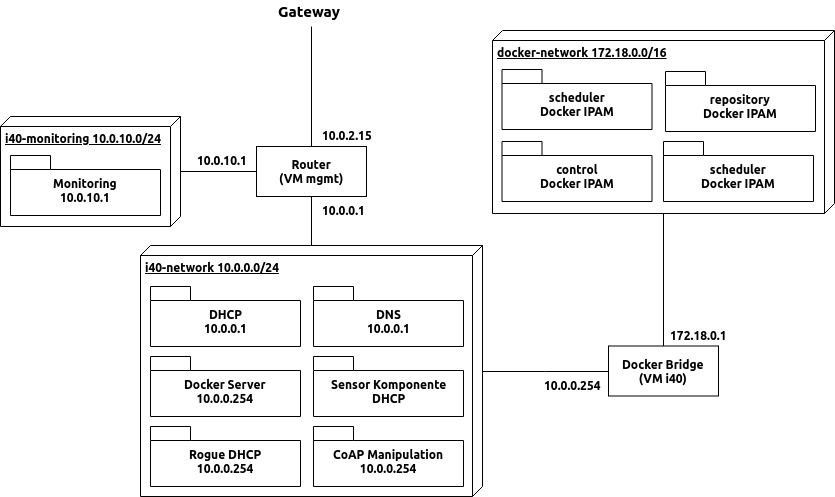
\includegraphics[width=15cm]{netzwerk}
  \caption{Netzwerkinfrastruktur} 
  \label{Konzept:Netzwerkkonzept}
\end{figure}

\clearpage

Die Kapselung und Sicherheit des Testsystems ist durch die Erweiterung um zusätzliche \ac{VM}s und Dienste weiterhin gegeben. Die Kommunikation mit dem Hostsystem und externen Netzen findet ausschließlich über die Netzwerkschnittstelle des Routers statt und dient der Installation und Konfiguration der Komponenten. Diese kann im Betrieb deaktiviert werden, um eine vollständige Isolation der Umgebung zu erzielen.

Durch die Konfigurationsmöglichkeiten der Hardware und des Netzwerks ist eine weitere Kapselung der Netzwerke mit Hilfe von \ac{VLAN} auf der Netzzugangssicht umsetzbar. Dies wird im Rahmen der Thesis jedoch aus zeitlichen Gründen nicht weiter bearbeitet.

\subsection{Industrienetzwerk}
Das Industrienetzwerk "`i40-network"' stellt den zentralen Bestandteil der Architektur dar. Dieses Netzwerk wird von den Diensten \ac{DHCP} und \ac{DNS} verwaltet und beinhaltet das Industrie 4.0 Produktionssystem und dessen Docker Sub-Architektur sowie die Sensor Komponente, welche Daten zum \ac{CoAP} Monitoring liefert. Der Netzwerkverkehr sowie die Verwaltung des Containernetzwerks wird vom Docker Dienst und dessen Netzwerkbrücke übernommen. Die Kommunikation mit dem Monitoringnetzwerk sowie mit externen Netzen wird mit Hilfe von \ac{IP} Forwarding und \ac{NAT} hergestellt. Der Rogue \ac{DHCP} Server befindet sich ebenfalls in diesem Netz und dient der Manipulation des für das Netzwerk \textit{authorativen} \ac{DHCP} Servers. Die Umsetzung dieses Netzwerks, der beinhalteten Dienste und der vollständigen Kontrolle über diese ist die Basis für die Durchführung der Anwendungsszenarien.

\subsection{Monitoring-Netzwerk}
Das Netzwerk "`i40-monitoring"' simuliert ein zusätzliches Netzwerk, welches Dienste zur Analyse und Überwachung der Komponenten im Netzwerk bereitstellen soll. Im beschriebenen Konzept besitzt das Monitoring-Netzwerk ausschließlich eine Komponente zur Überwachung der gesendeten Daten des im "`i40-network"' vorhandenen Sensors. Eine weitere Ausführung der Komponenten im Netzwerk hätte keinen Einfluss auf die gewählten Anwendungsszenarien (\autoref{Anwendungsszenarien:MitM} und \autoref{Anwendungsszenarien:Manipulation von ungesichertem Netzwerkverkehr}) gehabt, da die Kommunikation über ein Gateway der ausschlaggebende Faktor für die Integration des zusätzlichen Netzwerks war. Aus diesem Grund wurde auch kein \ac{DHCP} und \ac{DNS} für das Netzwerk konfiguriert. Die Adressvergabe verläuft statisch.

\subsection{Containernetzwerk}
Das Containernetzwerk beschreibt das grundlegende Testsystem und wird in \cite{Weber2018} beschrieben. Die bereitgestellten Container der Industrie 4.0 Umgebung werden durch den Docker Server verwaltet. Dieser übernimmt das \ac{IPAM} sowie den \ac{DNS}. Die Kommunikation zwischen den Container sowie mit dem Hostsystem findet über eine Software-Bridge\footnote{TODO - eine Bridge ...} statt. Diese Form der Netzwerkkommunikation ermöglicht es das Anwendungsszenario \autoref{Anwendungsszenarien:OPC UA Kommunikation} durchzuführen. Die Software-Bridge nimmt den gesamten Netzwerkverkehr entgegen und leitet ihn weiter. Somit ist es möglich diesen vom System, welches die Container verwaltet, zentral zu untersuchen.

\section{Bausteinsicht}
Die aus den Anwendungsszenarien (\autoref{Anwendungsszenarien}) hervorgehenden Anforderungen müssen durch die Komponenten im System umgesetzt werden. Hinzu kommt, dass die beschriebenen Netzwerke durch erforderlichen Dienste verwaltet werden müssen, um die Kommunikation der Komponenten zu gewährleisten. Die logische Darstellung der Verteilungssicht unterscheidet sich grundlegend von der Umsetzung der Komponenten in der Bausteinsicht. Die Virtualisierung der Maschinen erlaubt es mehrere Komponenten auf einem System zusammenzufassen und mit mehreren Netzwerkschnittstellen in verschiedenen Netzen auszustatten, um multiple Systeme darstellen zu können.

In \autoref{Konzept:Virtuelle Maschinen} werden die \ac{VM}s sowie deren Dienste und Schnittstellen in die Netzwerke dargestellt. Die Dienste \ac{DHCP}, \ac{DNS} im Netzwerk "`i40-network"' sowie die generellen Routingfunktionalitäten werden von der \ac{VM} "`mgmt"' bereitgestellt. Des Weiteren wird dort der \ac{CoAP} Server umgesetzt, welcher sich im Netzwerk "`i40-monitoring"' befindet. Die \ac{VM} "`i40"' beinhaltet die Komponenten zur Manipulation des Netzwerks sowie das Containernetzwerk. Der \ac{CoAP} Client des Netzwerk "`i40-network"' wird auf der \ac{VM} "`comp"' ausgeführt.

\begin{figure}[h]
  \centering
  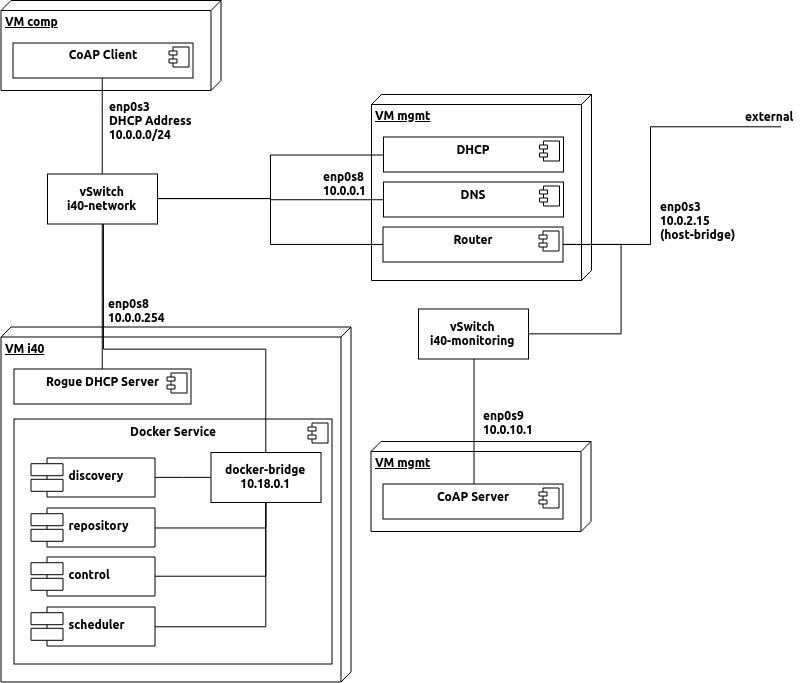
\includegraphics[width=15cm]{vm}
  \caption{Virtuelle Maschinen und Dienste} 
  \label{Konzept:Virtuelle Maschinen}
\end{figure}

\subsection{Router}
Die Routingfunktionalitäten werden auf der \ac{VM} "`mgmt"' umgesetzt. Die \ac{VM} besitzt in jedem Netzwerk ein Interface, welches als Schnittstelle dient und zur Weiterleitung der Pakete genutzt wird. Die \ac{VM} "`mgmt"' ist die einzige Komponente der Architektur, welche eine Verbindung zum Hostsystem besitzt. Die Weiterleitung der Pakete wird auf der Internetschicht des \ac{TCP}/\ac{IP} Referenzmodells mit Hilfe von \ac{IP}v4 Forwarding und \ac{NAT} umgesetzt. Durch das Routing zum Hostsystem ist eine Verbindung der anderen, gekapselten Maschinen sowie zukünftiger Maschinen für Installations- und Konfigurationszwecke in externe Netzwerke möglich. Um die Sicherheit des Netzwerkverkehrs sicherzustellen dürfen nur Pakete von Verbindungen, welche aus einem der internen Netze initiiert wurden weitergeleitet werden. \autoref{Konzept:Routerkomponente} stellt die Schnittstellen der Komponente dar.  

\begin{figure}[h]
  \centering
  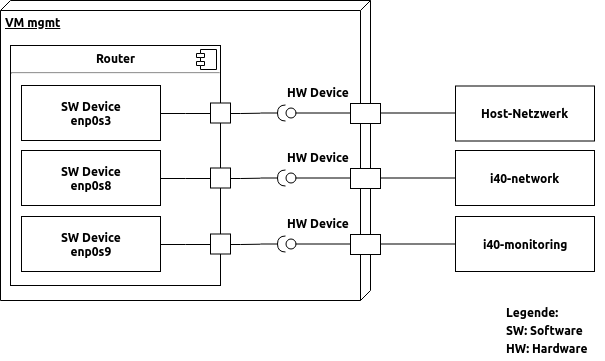
\includegraphics[width=15cm]{router}
  \caption{Routerkomponente} 
  \label{Konzept:Routerkomponente}
\end{figure}

\subsection{\ac{DHCP} Server/\ac{DNS} Server}
Die Dienste \ac{DHCP} und \ac{DNS} werden zusammen auf der \ac{VM} "`mgmt"' konfiguriert stellen ihre Dienste im Netzwerk "`i40-network"' bereit, indem sie auf die zuständige Schnittstelle gebunden werden. Zur Umsetzung der Anwendungsszenarien \autoref{Anwendungsszenarien:MitM} und \autoref{Anwendungsszenarien:Manipulation von ungesichertem Netzwerkverkehr} liegt der Fokus der bereitzustellenden Funktionalität auf dem \ac{DHCP} Server. Dieser muss den weiteren Komponenten im Netzwerk beim \ac{DHCP} \textit{discover}, welcher über einen Broadcast\footnote{TODO Broadcast} durchgeführt wird, eine Netzwerkkonfiguration bereitstellen. Dabei ist die Vergabe eines Standardgateways für die spätere Durchführung des \ac{MitM} Anwendungsszenario essentiell. Das \ac{IPAM} sowie die Konfiguration des \ac{DNS} und dessen dynamische Zonenaktualisierungen spielen bei der Umsetzung des Angriffs nur eine nebensächliche Rolle. Sie werden jedoch trotzdem umgesetzt, da die Konfiguration des \ac{IPAM} und der \textit{address range} der \ac{DHCP} \textit{leases} eine Möglichkeit gibt den Wechsel des \ac{DHCP} Servers zu Lehrzwecken visualisieren zu können. Die Bereitstellung eines mit dem \ac{DHCP} Server kompatiblen \ac{DNS} Servers vereinfacht durch die Namensauflösung die Verwaltung der virtuellen Maschinen in der Testumgebung und ermöglicht eine Skalierbare Erweiterung des Systems. Die Verwaltung eines separaten \ac{DNS} Servers ermöglicht die Umsetzung weiterer Anwendungsszenarien und die Analyse des Sicherheitsmechanismus \ac{DNSSEC} am Testsystem. Diese Anwendungsmöglichkeiten sind kein Bestandteil der Thesis und werden im folgenden nicht weiter erläutert. Sie bieten jedoch Ansatzmöglichkeiten für zusätzliche Erweiterungen am System und werden in \autoref{Ausblick} näher beschrieben.

\autoref{Konzept:DHCP und DNS Server} zeigt die Komponenten \ac{DHCP} Server und \ac{DNS} Server und die genutzten Schnittstellen in Bezug auf das Gesamtsystem. Beide Dienste werden auf das Netzwerkinterface des Netzwerks "`i40-network"' gebunden. Somit werden die Dienste ausschließlich im beschriebenen Netzwerk bereitgestellt.

\begin{figure}[h]
  \centering
  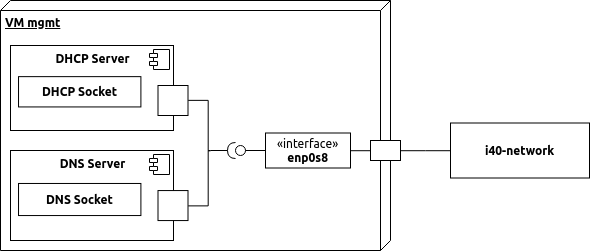
\includegraphics[width=15cm]{dhcpdns}
  \caption{DHCP und DNS Server} 
  \label{Konzept:DHCP und DNS Server}
\end{figure}

\subsection{\ac{CoAP} Client/\ac{CoAP} Server}
Die Komponenten \ac{CoAP} Client und \ac{CoAP} Server dienen der Erweiterung des Testsystems um ein weiteres \ac{IIoT} Protokoll zur Darstellung des in \autoref{Anwendungsszenarien:Manipulation von ungesichertem Netzwerkverkehr} beschriebenen Szenarios. Die Komponenten simulieren einen Temperatursensor sowie ein Monitoringsystem, welches ein Webinterface zur Darstellung der gemessenen Temperatur besitzt. Der \ac{CoAP} Client wird auf der \ac{VM} "`comp"' realisiert und befindet sich im Netzwerk "`i40-network"'. Er sendet die gemessenen Daten zum zuständigen \ac{CoAP} Server im Netzwerk "`i40-monitoring"'. Der \ac{CoAP} Server wird, da er den einzigen Dienst in diesem Netzwerk darstellt, auf der \ac{VM} "`mgmt"' bereitgestellt. Die \ac{VM} "`mgmt"' besitzt bereits ein Interface im Netzwerk "`i40-monitoring"'. Der Dienst kann auf die Adresse der Schnittstelle gebunden werden. Es muss keine weitere \ac{VM} zum Netzwerk hinzugefügt werden.

\autoref{Konzept:CoAP Client} und \autoref{Konzept:CoAP Server} visualisieren die Bestandteile der betroffenen Komponenten, deren bereitgestellte Dienste und die genutzten Schnittstellen.

\begin{figure}[h]
  \centering
  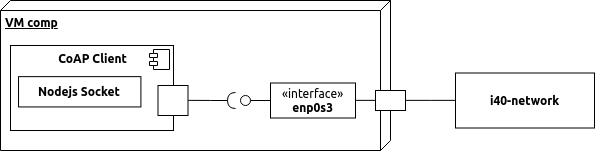
\includegraphics[width=15cm]{coapClient}
  \caption{CoAP Client} 
  \label{Konzept:CoAP Client}
\end{figure}

\begin{figure}[h]
  \centering
  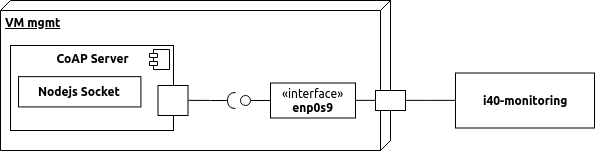
\includegraphics[width=15cm]{coapServer}
  \caption{CoAP Server} 
  \label{Konzept:CoAP Server}
\end{figure}

\subsection{Rogue \ac{DHCP} Server}
Die Bereitstellung des Rogue \ac{DHCP} Servers findet auf der bestehenden \ac{VM} "`i40"' statt. Die bestehende virtuelle Maschine stellt bereits Tools zu Analyse der Netzwerkkommunikation für das Dockernetzwerk bereit. Eine Erweiterung dieses Systems ermöglicht es die bereitgestellten Anwendungen zur Analyse in den Anwendungsszenarien des Netzwerks der \ac{VM}s ebenfalls zu nutzen. Dies wird durch die Trennung der Netzwerkschnittstellen ermöglicht. Die Analyse der Pakete findet fortan auf der Schnittstelle "`enp0s8"' statt der Docker Netzwerkbrücke statt. Um die Netzwerkpakete der anderen Teilnehmer über die Schnittstelle der \ac{VM} zu leiten, muss die Maschine selbst als Gateway für die Kommunikation zwischen den Netzen genutzt werden. Der Rogue \ac{DHCP} Server ermöglicht die Änderung des Standardgateways bei Erneuerung des \ac{DHCP} \textit{lease} der Client und kann somit den Verkehr auf das lokale System umleiten. \autoref{rogueDhcp} zeigt die Eingliederung des Dienstes in das vorhandene System. Der Dienst muss im Netzwerk "`i40-network"' agieren und wird somit auf das Interface "`enp0s8"' gebunden.

\begin{figure}[h]
  \centering
  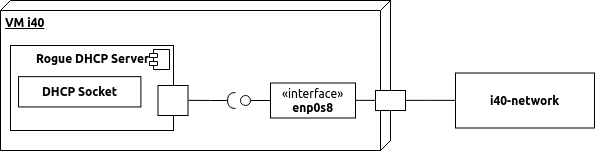
\includegraphics[width=15cm]{rogueDhcp}
  \caption{Rogue DHCP Server} 
  \label{Konzept:Rogue DHCP Server}
\end{figure}

\subsection{\ac{CoAP} Manipulationssystem}
Das \ac{CoAP} Manipulationssystem wird genutzt, um das \ac{CoAP} Monitoringsystem durch falsche bzw. unzulässige Netzwerkpakete zu beeinflussen. Es wird ebenfalls auf der \ac{VM} "`i40"' bereitgestellt. Dies ermöglicht die weiterhin die zentrale Verwaltung des Systems und die Durchführung der Anwendungsszenarien. Eine Bereitstellung des Manipulationsdienstes auf dem gleichen System wie der Rogue \ac{DHCP} Server und die Anwendungen zur Netzwerkanalyse ist sinnvoll, da die Umleitung der Netzwerkpakete durch den Rogue \ac{DHCP} Server und die anschließende Analyse des Verkehrs die Grundlage für die Manipulation des Monitoringsystems darstellt und voneinander abhängig ist.

Das \ac{CoAP} Manipulationssystem versendet Netzwerkpakete mit gefälschten Daten zum \ac{CoAP} Monitoringsystem. Diese werden über die Netzwerkschnittstelle "`enp0s8"' in das "`i40-network"' versandt. Die Verbindung in das Netzwerk "`i40-monitoring"' wird über die Routingfunktionalitäten der \ac{VM} "`mgmt"' bereitgestellt. \autoref{Konzept:CoAP Manipulationssystem} beschreibt den Aufbau der Komponente.

\begin{figure}[h]
  \centering
  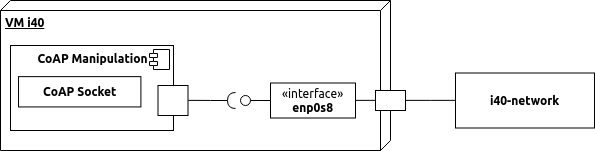
\includegraphics[width=15cm]{coapManipulation}
  \caption{CoAP Manipulationssystem} 
  \label{Konzept:CoAP Manipulationssystem}
\end{figure}

\subsection{Docker Service}
An der Netzwerkkonfiguration sowie am auf der \ac{VM} "`i40"' bereitgestellten Docker Service wurden keine Änderungen vorgenommen. Die genutzte Konfiguration des Dienstes ist in \cite{Weber2018} erläutert. Eine Integration der neuen Komponenten als zusätzliche Container im bestehenden Netzwerk war nicht möglich, da dies die Analyse des Netzwerks durch die Netzwerkimplementierung der Software Docker verfälscht bzw. verhindert. Eine genaue Beschreibung der Beschränkungen, welche bei der Umsetzung des Systems zum Tragen kamen, wird in \autoref{Konzept:Softwarebeschränkungen} durchgeführt.

\section{Laufzeitsicht}
TODO - Sequenzdiagramme
1. OPC UA Netzwerktraffic in Docker Netzwerk
2. CoAP Traffic mit DHCP
3. CoAP Traffic mit Rogue DHCP
4. CoAP Manipulation

\section{Anpassungen}
\label{Konzept:Anpassungen}
TODO

\subsection{Softwarebeschränkungen}
\label{Konzept:Softwarebeschränkungen}
TODO

\subsection{verworfene Konzepte}
\label{Konzept:verworfene Konzepte}
TODO